\textbf{Camp \emph{X-Ray} (-550 m): Inside the Hollow Mountain}

\textbf{Underground Camp Logbook Entries} \textbf{2011}



\textbf{Izgubljeni Raj 2011} **** \textbf{Revenge of}
\textbf{\emph{X-Ray}}

{[}The start of 2011\ldots{}{]}

\textbf{21/7/2011 1.45am} \textbf{Jan Clare, Miles, Jarv}

Arrived! 5 hrs down from the sunny plateau with 7 tacklebags, Jarv
(hero) rigged from Space Odyssey. Jan was pursued by a strange chicken
smell which turned out to be a split packet of Bachelors Chicken Savoury
rice. Jarv (weirdo) arrived at camp first (\textasciitilde 11.30pm)
imagining he'd find an emancipated caver\ldots{} instead there was a
carpet of mould growing on the debris of 2010. We spread sand on the
mold, broke out the comf. collected water, cooked food, set up the fairy
lights and cranked up the tunes! Aah yeah. Tomorrow we hope to recce
\emph{Serpentine}, limit of explo.

\textbf{10:20} \textbf{am} \textbf{Jarv}

Time to get up! reset my 9am alarm so we had a bit more of a snooze (the
Blackadder went off @ 2:30 am). Jan's bladder has dragged us out of bed
-- quite a tight callout, 10PM, so little time to explore.

\textbf{11:07 am (21-7-11) Clare}

Jan is cooking soupy cheesy smash while Jarv and Myles are lazing in bed
listening to Blackadder. I was dragged out of bed by my bladder but
since we didn't have a piss BDH I did a Tetley special and pissed into a
resealable bag instead. Dribbled over pants a bit but otherwise OK. Camp
is super comfy and I don't want to leave.

\textbf{11:22} \textbf{am} \textbf{Myles}

The morning after the night before. Awoke after slightly disturbed sleep
and thus forced to remain in my comf as long as poss. Clare pissed in a
bag, Jan cooked orange smash and we all listened to Blackadder. Camp is
5.3°C! Possible due to the biological processes of the mould
civilisation controlling camp. Now for a little bimble and then out for
tea and medals. WOOF WOOF.

\textbf{12:45pm 21-7-11 Clare}

Myles and Clare. Gone for a little bimble around Leopard. Aim to be out
for sunset. MP3 player died, think its out of battery. See you up top!
{[}Note by Jarv -- charge it with the speaker USB-battery thingy!{]}

\textbf{5pm 21-7-11 Jarv}

Saw Clare and Myles down Albert Hall/\emph{Serpentine}. Sniffed lots of
leads out with Jan:

1 Just after traverse on Consort Road (red rope). Dry oxbow on right
passage (narrow rift) goes back but doesn't intersect passage. Echo
suggests pitch/chamber. Good lead for small fresher.

2 Near Esoterica, waterfall inlet on left. Climb down between boulders
(easiest is to continue towards Albert Hall down mud slope climb then
double back into crawl), follow water sounds to undropped 10-15 m pitch.

3 \emph{Serpentine}/It will Rain. Follow red rope down from Albert Hall
-- at end of It will rain, fairly difficult 1.5 m cascade/freeclimb to
start of pitch. We rigged \textasciitilde 5 m to ledge, look down 10-15
m (nice pitch!) into what appears to be chamber (big ish). With water.
Left \textasciitilde 25 m 10 mm in tacklesack, also \textasciitilde 12 m
10 mm left @ end of It will rain.

Reheated tea and peanuts, time to head for surface!

Good luck team Thursday/Friday!

\textbf{22-07-2011 7:45 pm Tetley}

Johnny and Tetley arrived at \emph{X-Ray} after a smooth 4hr journey
down. It's good to be back! Fairy lights\ldots{} not so sure about
them\ldots{} Cup of tea then off for a tourist trip down Friendship
Gallery.

9:45 pm Arrived back from F. Gallery bimble to see Fairy lights\ldots{}
Ah\ldots{} already I associate them with all that's good about u/g camp!
Soupy cheesy fishy smash for supper.

\textbf{22.07.2011} \textbf{Not} \textbf{sure what time\ldots{}. Jonny}

First night at U.G. Camp! had a nice 4hr trip down to camp followed by a
quick trip to the Top of \emph{Big Rock Candy Mountain}. Tasty dinner of
cheesy soupy fishy smash. Lieing in a sleeping bag watching Blackadder
whilst Tetley tries to make \emph{Zimmer} nice. Camp appears to be
comfier than bivi! Looking forward to starting pushing tomorrow.

\textbf{23-07-11 2a.m. Tetley}

Yep left Johnny in camp to play on \emph{Zimmer} for 3hrs, hopefully the
new rig is better. Returned to find Johnny almost asleep. Listening to
some Bach. Sleeping pills for Jonny, Žganje for me!

``For us going to the toilet is a mundane activity, for you it is the
basis of an entire culture'' -- the Red baron (Blackadder).

\textbf{23-07-11 Tetley}

Woke up 10:15a.m. Setting off to push leads beyond Leopard 12:30p.m.
Discoveries await\ldots{}

\textbf{23.07/11 22:00 Jonny}

Just back from a nice pushing trip. Myself and Tetley headed to
\emph{Wonderland} -- hidden surprise, then kamikaze. After a short
hammer to make a squeeze bigger for me we followed a path next to
kamikaze and ended up in a larger chamber `The Red baron' (see previous
page). We surveyed the area; promising lead, traverse across
\textasciitilde 5 m drop. Left the lead to check the end of kamikaze.
Turned out to be a ``COLLECTOR'S PIECE'' (Tet) i.e.~a crawl. End was
blocked although sound of RUSHING WATER was very clear and a passage
could be seen through boulder -- exciting. Trip back was a bit arduous;
dehydrated. Made it back to camp for a great pint of tea, blackadder and
the roar of \emph{Zimmer}. Storm possible up top? Still -- interesting
leas, possibly a horizontal continuation? Making food -- nice cous cous
and sausage.

\textbf{23:00 23-07-2011 Tetley}

Top tip \#1 Don't take Žganje and then take sleeping tablets.

Top tip \#2 If you go to push the exciting lead off Red Baron, take some
water with you to drink!

75 m surveyed today, most in `Red Baron', a big chamber. Many thanks to
DW and JKP for leaving us the storming and draughting lead, complete
with a PSS at the start!

{[}Tetley's sketch of Red Baron chamber{]}

The lead: rope traverse needed over 5?m drop, horizontal passage awaits!

\textbf{23:58 23/7/2011 Tetley}

Went to empty piss BDH -- still a lot of water coming down
\emph{Zimmer}.

\textbf{9:45 am 21/7/2011 Tetley}

A good night's sleep, no headache this morning. Tea and Dangerous Dick.
\emph{Zimmer} is still very wet -- no other cavers have come to join
Jonny and me. I'm in a great mood, Jonny is perhaps apprehensive about
the climb out.

10:30 a.m. We've decided that \emph{Zimmer} is too wet to start
out\ldots{} so we'll be staying warm and dry at Camp \emph{X-Ray} for a
while. The bad news is that I'll have to take a shit. grrr.

\textbf{10.33 am? 27/7/2011} \textbf{Jonny}

Avoiding going up \emph{Zimmer}, flood pulse? Staying at underground
camp listening to music until a reasonable time to get out. May do some
bolting practice? here's hoping that \emph{Zimmer} decides to dry up a
little sooner rather than later

\textbf{24/7 14:45 Tetley}

It's still bucketing down \emph{Zimmer}! Jonny and I are still alone,
Jonny has now broken through the 48hr barrier. We've moved to half sugar
rations, oh life is tough!

\textbf{24.7.11 16:15 Jonny}

Amazing what putting in a single bolt can do. Moral boosted slightly
after contracting a bit of `the fear' and speaking to Tetley about
stories of broken pelvis', rescues and general caving deaths.
\emph{Zimmer} still pissing down so we'll wait until morning before
making ascent, be it wet or not.

{[}Small cartoon by Jonny showing a wet pitch{]}

More interestingly, seems like the stream near camp \emph{X-Ray} is
likely to be separate

from the \emph{Zimmer} -- water seems to come from opposite direction
(Obviously due to large amount of water). ``Now don't tell me I've
nothing to do''

\textbf{24/7/11 18:20 Tetley}

After an hour of `Dead Ringers' we've moved on to `Little
Britain'\ldots{}

21:25 Jonny and I have both been dozing, still no sign of other cavers,
what's going on `up top'???

23:30 Clare and Jarv arrived at 10:40pm with tales of apocalyptic horror
on the surface -- snow! storms etc. Looks like Jonny and I made a good
call!

23:38 Clare and Jarv gone to push lead off Red Baron -- back to sleep
for Jonny and me.

\textbf{25.7.11 9am} \textbf{Jonny}

C+J arrived back around 7:30am having found \textasciitilde 200 m of
cave. Tetley and myself now off to the surface. Little apprehensive to
leave the comfort of camp but after three nights it's time to leave!

\textbf{25/7/2011 9:05 a.m. Tetley}

Final faff/fag before heading out. Many thanks Jonny for an excellent,
productive, fun 3 night camp -- looking forward to the Laško I left at
the entrance

p.s. Thanks to all who've made \emph{X-Ray} so pleasant -- Jarv
especially.

\textbf{25-7-11 10pm Clare}

Clare and Jarv. Arrived at camp yesterday night and left immediately to
push Red Baron after a chat with Tetley and Jonny. Found
\textasciitilde 220 m of passage we named `The Throne Room' on an 8hr
bolt pushing trip. New Uneo finally worked under Jarv's loving touch!
Night train is hard work though -- caving on autopilot on return to
camp. Now in bed listening to Blackadder over coffee and ready munch.
Jan and Kate, Dan and Myles were supposed to have arrived on the day
train a few hours ago to kick us out of bed but no sign of them. Where
have all the cavers gone?

\textbf{25-7-11 10:30pm Jarv}

Jan and Kate arrive! Nice to see some other peeps. Strange condensation
on the sleeping bag -- perhaps we can dehumidify the whole tent with
carbide?

Mornings in UG camp are a perpetual Sunday Morning. We had chocolate and
latte in bed. It was rather nice.

I think I slept 8AM -- 8PM ish, with a little break for a piss and a sip
of water. Clare was making little sleepy noises, like a rabbit, but
apparently slept little.

The drill is much fun, v quick and efficient.

{[}Little cartoon by Jarv of him and Clare bolting{]}

Place 8 rawl bolts with the tiny 10-cell Nimh battery.

{[}Jarv's sketch of the Throne Room{]}

Strong draught over traverse, mostly disappears after climb (stations
1-8). Suspect goes into window, about 4-5 m above PSS.8 in chamber. Easy
climb but should preferably protect with bolts. Might be easier to
traverse back from .8

{[}Jarv's sketch plan of the Throne Room{]}

{[}Jarv's cartoon of Kate and Jan cooking{]}

\textbf{27-7-11 1am} \textbf{Jarv}

Jarv and Clare. Finally off -- to push Round Pond! callout Noon 26-7-11,
should be back earlier to cook some breccy for K \& J. See ya!

\textbf{26-7 Jan}

Arrived after \textasciitilde 10pm waking Jarv and Clare, who were happy
to see people. Had food and tea, went to bed after Kate danced to Duran
Duran. Jarv and Clare set off to \emph{Serpentine}. Slept well, woke
9am. Jarv arrived, had tea, Mexican rice + coffee.

\textbf{26-7-11 Noon Jarv}

Ensconced in the comf, watching Kate \& Jan get ready. Today we did
pitches -- pushed round pond → The Long Water. 40 cm straws in first
chamber, way on via boulder choke then pich up water to small 6 m pitch.
Follow stream to cascade chamber -- very pretty. Water goes down a
pitch, also climb to b/choke (a bit small for humans) which prob goes to
same pitch. Also, Clare found `Rotten Row', continue past the first
little dried pool with pretty grey sediment into body-sized phreatic
which leads after a few twists to another pitch. You can see 10 m down
onto ledge. Big sound of water but no sign of it.

Good stuff! Left tacklesack with \textasciitilde 50 m of 10 mm at foot
of 2\textsuperscript{nd} pitch, before cascade climb.

\textbf{26-7-11 10pm Jarv}

Woke at six \& couldn't get back to sleep, accepted this reality at 8 \&
got up to warm some vitaminski in time to receive Myles and Mike. Sent
them off in the direction of Kate \& Jan.

\textbf{27-7 10 50 am Jan}

Woke for a piss after a warm nights kip, Kate, Michael + Myles also in
residence at Chateau \emph{X-Ray}. Yesterday I spent 3.5 hrs bolting
across a traverse at \emph{Cheetah}, Kate waited patiently at top.

{[}Jan's sketch topo of \emph{Cheetah} traverse. {]}

The last thru-bolt only went in halfway, so the Spirit of Elvis was with
me as I scrabbled for a foothold and reached for the lip of the
window\ldots{} and my light shone to the back for the first time, sadly
it wasn't another exhibition Road but the bottom of a cascade. Still an
exciting traverse nonetheless!

We did a tourist trip to Red Baron chamber then back to camp, meeting
Myles and Michael. Watched RARG on the video player with Jarv + Clare +
Kate in a cosy ball of comf.

\textbf{27-7-11 11:30} \textbf{am} \textbf{Myles}

Mike and I arrived last night and after a brief visit to camp, went to
look at Throne Room. Nice cave! When we returned to camp we found 4
comf-covered creatures refusing to leave! I cooked 7.3 Kg of smash for
Mike + I before settling in for bed. I had a ``Goonies'' style dream,
and now Kate is cooking breakfast\ldots{} Hopefully we're off to push
\emph{Serpentine}.

\textbf{Weds 27 July? Kate}

Yo Yo Yo. Jan \& myself are pushing Throne Room, expect to be back by
10, callout 12. Same times for Mike \& Myles who are \emph{Serpentine}
way. Lots of love Kate.

\textbf{27/7/11 Mike}

Mike + Myles. Leisurely start at 1 ish and headed off to
\emph{Serpentine}. Admired the extra pitches dropped since last year and
followed Jarv's directions to Rotten Row. Looked at two pitches and
bolted the easier one with natural back up.

{[}Small topo by Mike{]}

Water headed on down, small hole + climb on left or follow water (1.5 m
drop). Next pitch approx. 30 m? -- Didn't descend whole way. Bolt on
floor+ rigged off natural + dropped \textasciitilde 10 m Wet so swung
over and ascended.

{[}Another small sketch topo by Mike{]}

Derigged all as neither of us were happy with it. 50 m of 10 mm and
\textasciitilde 10 m of 10 mm left at top. Returned to camp 8:30 ish
after quick survey.

\textbf{Thurs 28/7/11 11.15am} \textbf{Jan}

Jan and Kate. Just contemplating heading out. Had a great trip down The
Throne Room yesterday came back to camp to find Myles + Mike in bed
after an equally exciting push down \emph{Serpentine}! Lots happening

We did two climbs in The Throne Room which lead to a storming passage
called `\emph{Amazing Grace}', after Kate played it on the harmonica
while I climbed, thanks Kate! You took my mind off the scariness +
rapture.

{[}Jan's sketch of \emph{Amazing Grace}{]}

A good draught is going down `\emph{Amazing Grace}'\ldots{} We turned
round at a muddy climb so someone else could enjoy the push too! Go! Go!
Go!

\textbf{24/7/11 Kate} \textbf{{[}Incorrect date!** **{]}}

My hands are extremely fucked so this may be short. Had a wonderful few
days underground. Camp is as lovely as ever. I've even taken to eating
smash which I thought would never happen after the incident with the
sleeping bag last year.

Had two pushing days, the first of which, despite Jan's heroic effort,
was not so successful although we did answer the unanswered potential of
the window off \emph{Cheetah}. Later that day after sitting at the top
of \emph{Cheetah} freezing my bollocks off we went to find the location
of the Red baron and the pushing front where Clare \& Jarv had an
uninvestigated window.

It was on Jam and my second pushing day that we went there. After much
prodding around Jan climbed and bolted a window above the Throne Room.
Meanwhile I played Jan's harmonica. Annoying we found this window led to
a small passage running parallel to the easily accessible passage in
which Jarv had a shit and that these passages connected via a small
crawl. There was however another window as well. Jan climbed and bolted
this one which led to a wide horizontal passage. We excitedly stumbled
up the passage which then turns 90° to a downward slope. Quite nice and
passable with mud resembling bird poo coating the rocks. With time
running short and Jan wanting to leave it open for the next team (this
want I did not share) we stopped at a muddy easy climb. Could see
another 15-20 m but after there who knows.

It's wide, it's horizontal and it's blowing so what are you waiting for?
Go discover some motherfucking cave! Leaving now, Love Kate.

{[}Small cartoon/sketch by Kate{]}

\textbf{27/7/11 Izi}

Izi, Kletnik (nočna ptiča) **** Sva šla plezat okna v Albert Hall in
Minotaur rift ni blo uspeha. Pol sva šla pa v \emph{Serpentine} zlezla
okno in po kratkem rova dobila majhno brezno na dnu po blatnem rovu
naprej do večjega\ldots{} se nadaljuje (kletnk je predebel). Novi del se
kliče: Let na drugi svet

Camp was perfect!

Hope to be back soon.

HVALA ZA USE

{[}Sketch survey of Let na Drugi Svet{]}

\textbf{29/7/2011 4pm Tetley}

Back again -- smooth sub 2 hr trip down. Good to see Izi + Samo. Off now
to \emph{Amazing Grace}. Tetley and Clare

\textbf{1:25 am 30/7/2011 Tetley}

Clare and I have returned with 260 m in the book -- the new find, after
\emph{Amazing Grace} is called the \emph{Magic Dragon}! Gergely + Jana
also here, in bed, Jarv + Dan off pushing -- more tomorrow after sleep!

\textbf{8:30 a.m. 30/7/11 Tetley}

Dan + Jarv have returned, listening to Ella Fitzgerald, reminiscing
about our great day yesterday\ldots{}We rerigged Jan + Kate's
`\emph{Amazing Grace}' climb (see 3 pages back) so now the `abandoned
climb' is connected to serenade PSS7.

{[}Sketch survey showing cave from Red Baron to the \emph{Magic
Dragon}{]}

\textbf{30-7-11 23:58 Jarv}

Night train Jarv and Dan. Tet \& Clare finally back from pushing below
\emph{Republika} -- starting to get worried. Mike, Z \& Stane passed
during the night -- first at 3pm to drop stuff off \& check in, then at
5pm to say goodbyeee! Stane popped back to take a photo of the tent, and
then off. Nice to see them all, but disturbed sleep.

Yesterday we visited \emph{Magic Dragon} -- nice crystals/quartz.
Degraded rather horiffically after PSS.1 ; we started to bolt the pitch
but the rock was appalling. Broken \& soft, quartzite broke the Spitz
teeth. Got a bolt in \& natural back up, went over the edge in the
horrific muddiness. The obv natural over the edge turned out to be mud.
The whole pitch lip in fact sticky mud \& white cheesecake boulders.
From the position I was in, sliding around with nasty muddy 9 mm, I
plumbed the depths -- 15.5 m \& then we bowed out. Slow return with cold
SNOOZES on the boulders to not be too early.

00:17 Jana's here! Tales of horrifically muddy pitch leading to massive
pitch.

Tet \& Clare have left `Daydreamer' at a nice lead above a pitch in
stream.

\textbf{01:45 31/7/2011 Tetley}

Another top trip! Clare and I went down to push below \emph{Republika}.
Dropped 3 pitches and a climb, left big lead -- nice 15+ pitch going
down, white rock, nice stream. Surveyed about 75 m, PSS at end. DON'T go
there if water levels are high. \emph{X-Ray} → pushing front about 3hrs
ditto for the return journey. It's going, going, going!

p.s. Our new finds below \emph{Insomnia} pitch are called
\emph{Daydreamers}.

\textbf{01:56 31/7/2011 Gergely}

Good pushing trip today with Jana at the end of the \emph{Magic Dragon}!
We named the pitch `\emph{Stuck in Paradise}', referring to the muddy
awkward terrible nature of it. At the bottom there are two ways on, one
pitch is dead while the other drops to something big, big wind and echo.
It gonna be hard to push though because all you SRT kit is just a big
lump of mud! It will be fun\ldots{} Nice new extensions, big sizes,
crystals and so on. Good to be back. I wouldn't have thought last year
that \emph{Wonderland} will lead to such big things! To the new
extensions, Gergely.

\textbf{29.7 -- 31.7 2011 Jana}

Jana + Gergely. Started late from the surface, we only had like 4hr
pushing. We pushed a small -- on the right bottom -- first chamber at
the beginning of Prince Albert Hall. Small passage went for about
\textasciitilde 30 m. Did a small climb and looks it goes on. Climb not
safe to check. Overall not a massive great lead. After we went to
\emph{Serpentine}, where we checked Samo + Izzy's push. Also de-rig the
original rope at the beginning of \emph{Serpentine} as it got fucked.

Back at camp and soon Clare + Tet joined, followed by Jarv + Dan (night
train). \emph{Amazing Grace} goes and pushed to the \emph{Magic Dragon}.
Clare and Tet stopped at a \textasciitilde 15 m pitch, which Jarv + Dan
decided to push. Sleeping time!

Woken up by Jarv + Dan, muttering about a muddy, horrid pitch. They
could not descent due to mud and then run out of time to bolt around.

Gergely and I decided to push it plus see all the new stuff. Clare + Tet
went to push \emph{Insomnia}. \emph{Amazing Grace} + \emph{Magic Dragon}
is super pretty. Loads of crystals again. The pitch to push is super
muddy indeed. having a drill made job a bit easier and Gergely did a
great job. At the bottom pitch splits in two by rock bridge. One way
dies (sort of -- a climb?) and other is a big pitch
(\textasciitilde 50). We named the place ``\emph{Stuck in Paradise}''.
Was so muddy you could not see your kit. Not very pleasant SRT. On the
end was completely covered in mud and looked like one big mud blop. Ha,
ha.

{[}Sketch survey of \emph{Stuck in Paradise}{]}

\textbf{31/7/11 11:17am Clare}

Amazing two pushing trips with Tetley down \emph{Magic Dragon} and
\emph{Daydreamers} -- \emph{Vrtnarija} is now deeper than ever before!
Put in my first bolts and properly dropped first pitches; cheers Tet for
an incredible camping trip and great company. Top tip: hot brews at -800
m is the absolute dogs bollocks. Now all that's left is a final prusik
to the surface. I hope Tetley goes nice and slow! he chased me up Big
Rock yesterday. Till my next camp, happy pushing to all.

\textbf{31/7/2011 Tetley}

So, July draws to a close, as does another great camping trip. Thanks to
Clare, you've been great. Looking forward to sunset and entering
\textsuperscript{1}/\textsubscript{3} km of survey data.

\textbf{31/7/ 18:30 Jana + Gergely}

After a muddy project yesterday, a muddy digging project today, where
again left at the top of the pitch. Great stuff, Jana

Good pushing and have fun. Watch out for the rapture. Gergely

\textbf{31/7/2011 Gergely}

Two digs at Friendship Gallery (don't turn left after the rope, but keep
straight on). Upper one needs explosives; bottom one -- the `Lower
Pleasures' leads to a pitch (cca 20 m). Quite good draught, a bit tight
(no SRT kit). Direction \textasciitilde 210°. To get to \emph{Lower
Pleasures}, climb down between boulders next to the PSS in the last
chamber of Fri. G. It goes slightly towards Sys Mig; but worth giving a
check for the wind also watch out at the end, don't fall down the pitch

{[}Gergely's small sketch of \emph{Lower Pleasures}{]}

\textbf{1-8-11 Jarv}

Jarv and Dan. What a sleep! From 2pm -- 10:30 am, Wowser. However with
our surface callout in less than 24hrs and us having failed to delay it
we must head out today.

Yesterday we worked on the pitch below Long Water. Didn't much like the
wet way pushed by Myles \& Mike, we went off Rotten Row.

{[}Jarv's ext elevation of pitch{]}

{[}Jarv's plan of pitch{]}

Suggestion to keep on rigging is to keep on deviating on left wall, then
bounce to right wall into continuation of rift for the final hang.

The Y-hang gives a perfect hang to the spray lashed ledge -- one could
just throw caution to the wind \& zip down, slam in a bolt in the wet
and continue.

The rotten row PSS 1 was knocked off its corner, I hid the label in the
roof -- it sits on the little ledge on the right about halfway down the
traverse.

{[}Jarv's small diagram showing location of Rotten Row.1{]}

\textbf{1-8-11 12:40pm Jarv}

Much dead ringers later, and a spot of lunch \& it's time to go. We're
both pretty stiff \& sore -- getting so cold on the wet pitch \& the
caving back to camp clearly isn't good for the body. Water levels still
very low -- I hope someone gets down in time to push \emph{Daydreamers}
and Longwater before it pisses down again!

Excellent clear up operation by the previous two teams -- little left to
take out so we'll tidy up a little, photo inventory \& the elopc (After
some hot vitaminski)

Good luck team August!

Get the bolts \& the metres in!

\textbf{1.8.2011 21\textsuperscript{00}} \textbf{Tjaša}

Grega \& Tjaša. We are going down the stuff (Let na drugi svet?) which
found Samo and Izi. We did some digging and heard a loud water noise.
There was a big draft. We came to water but we had no time to check its
way (we leave it for next day probably). Night!

\textbf{2.8.2011 22:00 Karin}

Nejc \& Karin. We came down around 4:00 had some tea and then we went to
Lower Pleasure. We tried to bolt it but we just couldn't. We came back
and sleep. Nejc is sick so we're going out. There is some rope in Lower
Pleasure left (I think 2 pieces about 10-20 m long).

\textbf{3 August 20:30 (morning) Gergely}

Yesterday we went climbing to the Queen's bed chamber. No good luck, the
layers of good rock are separated by muddy layers which are unsuitable
for anything really. Despite the heroic efforts of Izi, he managed to
climb about 7 m and came down. We left a rope in for further attempts
(which may involve some mud-stick operation). The window on the left
seems to be going.

Strangle, that now there was no wind at all in the end of Minotaur rift,
although last year it was a huge draught there. The reason may be the
difference in the water level. Today off to \emph{Stuck in Paradise}!
Good luck, Gergely.

\textbf{3 August 2011 Jonny}

Jonny + Dave. Arrived 9 o'clock last night after faffing all day, 3
hours down. Woke at 8 this morning and set off to tackle Big Rock candy
mountain. I sat shivering whilst Dave bolted wind; too muddy, taking too
long, Headed down; nasty rebelay but looks like a large parallel
chamber/shaft! Same dimensions as BRCM. Too late, let someone else climb
up.

Camp super comfy and I feel very comfortable; no rapture

{[}Jonny's sketch of \emph{Big Rock Candy Mountain}{]}

\textbf{{[}Here ends the original white covered logbook -- all the
following entries are from the red covered supplementary logbook{]}}

{[}Sketch by Tjaša/Karin showing things to do{]}

\textbf{4.8.2011 9:50am? Jonny}

Jonny and Dave. Fairly restless sleep but here I am, awaiting the
departure to the surface. Despite not discovering much yesterday, it's
been a great trip, especially experiencing some expedition bolting
(cold) and de-rigging (fun). Hopefully I'll be back in the next week,
even if it is for a de-rig. No sign of Izi + Gergely on the night train
-- hopefully they've found something exciting at \emph{Stuck in
Paradise}.

\textbf{5/8 -- 10:30 ish Mike}

Mike + Ari. Have just eaten my body weight in couscous (Dave decline
b/fast) and am both Happy + Sad. Off to go caving down the push on
Friendship Gallery soon.

\textbf{4/8/2011 13:20 Gergely}

Just got back from a good pushing trip with Izi. We found about 500 m of
new passage at \emph{Stuck in Paradise}! The rest of the pitch is the
same as the top: a muddy slopy loose-rocky thing. I thought
\emph{Cheetah} was horrible; but now I was glad to come back after
\emph{Stuck in Paradise}. The bolting was fairly OK with some
compromises; the who pitch -- especially the top -- is quite loose, and
it should be 1 person at a time! At the lower bit, the rocks come down
at the clear rock section, watch out.

At the bottom of the pitch a phreatic tube starts. This is similar to
Friendship Gallery in size. Plenty of crystals, very nice walking
passage for about 300 m. Then a boulder choke blocks the way, but we
almost managed to climb through in the middle -- there is a crack
between two large boulders which is just too small because of a ledge in
one of them, about 10cm big. This needs a chisel or capping. The passage
seemingly continues on the other side. Watch out for crystals please!

The other passage opens on the left of this one, it is quite low, but
this is the one that sucks the wind. Generally it is about 4 m wide, but
filled with mudstone, and not higher than 1 m (usually less). We
followed it for about 150 m. At the end there is a boulder choke, which
seems passable on the top, but we ran out of time. Strong draught!
Crystals here too and STALAGMITES: about 5 stal columns about 20cm high,
5cm wide. I think both of these are very good leads, although getting
there takes effort -- this adds to the fun though!

Meanwhile it turns out that we left the instruments \& survey book
somewhere, so tomorrow we have to go back for it. Part of the
fun\ldots{}. Good pushing, Gergely.

ps. The rope in \emph{Stuck in Paradise} is exposed to rockfalls, be
aware!

ps2. The longer passage is called Lost Miles, the windier is
\emph{Penitence}.

{[}Gergely's \emph{Stuck in Paradise} rigging guide{]}

{[}Gergely's sketch survey showing extensions below \emph{Stuck in
Paradise}{]}

\textbf{5/8/2011 13:00 Tetley}

Clare and I set off down GW at 9:30am yesterday. Smooth journey down,
meeting Dave + Jonny in Pink. Izi + Gergely were at \emph{X-Ray} with
exciting news of 500 m of new cave. ``Do you want to see the book?''
says Izi. NO BOOK! They left the survey book back in \emph{Magic
Dragon}\ldots{} One for them to sort out, Clare + I were on a mission to
\emph{Daydreamers}. Dropped 3 pitches there, but at the bottom of the
last one the water disappeared down a bedding plane crack\ldots{} Grr,
still I said we'd find a bypass and we did. Left a good drafting lead,
`The Penguin's Egg'. Met Fratnik, Jarv + Jim at Red Cow. Back to
\emph{X-Ray} for some much needed sleep. Thanks again Clare, 140 m in
survey book.

\textbf{5/8/11 9am} \textbf{Mike}

Mike + Ari: below `Lower Pleasure', ``2\textsuperscript{nd} Time Lucky''

Went back Fr. am to drop our pitch with correct length rope. Epic faff
on my part which Ari did well to put up with.

{[}Mike's plan of Lower Pleasure{]}

Two windows down pitch. 5 m drop with water at bottom and rift going
over 5 m drop. Tightish but air fresh -- no draft. Sorry Ari! Happy
caving all.

\textbf{5/8/'11 15:30 Tetley}

Clare + Tetley heading off to \emph{Penitence}, below \emph{Magic
Dragon}

\textbf{6/8/11 Midnight Jarv}

Jarv, Jim, Fratnik. The sun sets on another day train! Karin \& Samo are
already snoozing in bed, we are awaiting the return of Tetley \& Clare
while carrying out experimental cooking research.

Pretty tired and stiff after our long trip yesterday -- we went to find
the Penguin's Egg on our Winter Journey.

{[}Jarv's sketch survey of Winter Journey{]}

Draft follows squeezes in inclined bedding, eventually wind disappears
into ceiling rift. Heavy silt deposit in lower region of chamber -- near
backing sump? Mud stalagmites on rocks.

\textbf{6/8/2011 9a.m. Karin}

Samo \& Karin. Let na drugi svet -- Krtkova Dobra Dela -- Heroj
Telemarka\ldots{} \ldots{}BAM! Samo fell, so we're going out now. He had
``luck'' that he fell in water. There are 3 leads with water way, 2 up
\& 1 down.

{[}A sketch survey by Karin{]}

\textbf{6/8/2011 4:20 a.m. Tetley}

Firstly, respect to those, especially Gergely, who pushed Stuck in
Paradise. Amazing push\ldots{} truly heroic etc. Praise to to the
electric drill!

Clare and I went down to push the extensions beneath. We dug through the
boulder choke at the end of \emph{Penitence} to find Salvation -- 200 m
of mostly walking horizontal passage. Drafting lead left. Forgot to take
water, despite my own `top tip' early this expo, hence pretty dehydrated
after 10 hrs caving, no water to be found. Grade 1 survey to follow
after sleep. A great day, only marred by news of Samo's injury, I hope
he's OK.

\textbf{6/8/2011 9:45a.m.} \textbf{Tetley}

Note re: \emph{Stuck in Paradise}

Only one person should be on the pitch at a time. It takes 30-40 minutes
to ascend or descend.

If you shout `rope free' at the top, you won't be heard at the bottom
and vice versa\ldots{}\ldots{}.

\textbf{6/8/11 9:50 a.m. Tetley}

Tjaša and Eric here after coming down and pushing on the night train.
Samo, Karin and Fratnik heading out soonish.

{[}Tetley's sketch of Salvation{]}

\textbf{6/8/2011 1:20 pm Clare}

Another camping trip drawing to a close, quite probably my last pushing
trip of the expo! Just waiting for Jarv and Jim to return before we
start our bid for the surface. Once again, two successful pushing trips
down below \emph{Daydreamers} and in the kamikaze extensions below Stuck
in Paradise. Another 340 m in the book, and caving with Tetley's always
a pleasure. Special thanks to Gergely \& Jana \& Izi for bolting and
rigging and surveying the worst pitch in the world (\emph{Stuck in
Paradise}) so beautifully. We left a strong, draughting lead in
Salvation below the pitch, go push it!

\textbf{6/8/2011 13:30 Tetley}

Time soon to head up for tea + medals. Another great trip!

\textbf{6-8-11 22:00 Jarv}

Jarv \& Jim. Another glorious morning down @ Camp \emph{X-Ray}! Well, it
is night but who cares? Only hit the sack @ 16:00, thanks to sliding
forward in sync with Tet \& Clare.

Just had a strange dream for caving -- searching amongst Hipster pubs in
London with Jim; we were looking for other cavers but mainly for
1\textsuperscript{st} class toilet facilities. Here, alas, the piss BDH
is full.

Yesterday we went to the \emph{Serpentine} to try \& drop the wet pitch.
Didn't quite make it -- needed a rebelay \& found a natural but it was
just too dodge for the swing I'd undertaken. Jim was also shivering in a
sleeping bag, where I'd swung too was wet \& NO PLACE TO HAND BOLT.
Perfectly possible to rig this pitch dry, but requires a fair bit of
swinging \& a fist full of bolts.

{[}Jarv's sketch of `Drink Your Own'{]}

Anyway, having made a stab at it, and grabbed a few quick photos of the
straws in Longwater we withdrew gracefully.

Well, actually that was bollocks as we derigged the whole pitch series
\& found ourselves with three tacklesacks + a bolting kit through the
\emph{Serpentine} meander. Pretty epic, as one was a massive `Big
Bertha' sleeping bag tacklesack stuffed to the brim with wet 10 mm \&
metalwork. Still, made it to Friendship for 2pm, having left @ 5am. A
few plates abandoned in-situ, as rawl threads damaged by hammer.

{[}Jarv's sketch of \emph{Serpentine} pitch rigging part 1{]}

{[}Jarv's sketch of \emph{Serpentine} pitch rigging part 2{]}

{[}Jarv's sketch of \emph{Serpentine} pitch rigging part 3{]}

\textbf{6.6.2011 23\textsuperscript{00}} \textbf{Tjaša}

{[}For the next few entries, the recorded month changes, from 8 (August)
to 6 (June)!{]}

Erik \& Tjaša. We are going surving (?) The new parts around Krtkova
Dobra Dela we founded yesterday Kletnk \& Karin and if we will have time
do some pushing there. Lep pozdrav!

\textbf{6-6-11 22:50 Jarv}

Jarv \& Jim. Well, we've had Hippy tea \& a blast on the music player.
The gizmo is recharging \& we're going to try and get a little more
shut-eye before departing.

\textbf{7-6-11 13:00 Jarv}

Well! A bit more shut-eye turned out to be more than anticipated!

Erik \& Tjaša came back very quickly from surveying -- they got cold \&
wet and crawled into bed with us!

A very long sleep but worth it. Jim is feeling a lot less stiff \& my
back is popping less. Certainly the derig yesterday exacted its toll.

Camp is looking rather bare, nil shitbags, meths, sugar, hot choc, rice.
The train is crashing \& it's time to get off.

\textbf{14:48} \textbf{Jarv}

Good luck Erik \& Tjaša, see you on the surface!

\textbf{7.8.2011 17\textsuperscript{00}} \textbf{Tjaša}

We were surveying and get very wet. We had surved Heroj Telemarka that
found Samo \& Karin yesterday. Samo falls into the waterand there is
also our surveying stopped. That is on the left side (part on Karin's
drawing where are ``two amazing lakes''). Then we went to the right.
Karin had written that there are 2 meanders but is only one. It just
looks like there are 2 because they're one above another but after a few
metres they become one. That meander ends after 30 meters. There is
water so we couldn't get over it. I think it is possible but you get all
wet. So we end after 30 meters. We do the last station on a rock wich
looks like this but we didn't put any paper because it hangs from the
cealing (strop -- SLO).

{[}Tjaša's sketch referred to above{]}

We decided that the name will be the same as Karin \& Samo gave it to
the nearer part and because they told us to go there. So, it's named
Heroj Telemarka.

We eat 2 frutabelas there and go surveying the part which founded I and
Grega few days ago (that little canyon). We named it Krtek in Orel. The
last station is above the bigger pitch. We didn't surved it down because
we didn't want to get wet. Anyway, when we went back + swing on a rope
accidently under the waterfall and get wet. And Erik get wet in the
squeeze in Krtkova Dobra Dela. So, we were all wet in the end.

Shit happens : )

Under the bigger pitch Erik bolted something and it's possible to go
down. If you follow the water you come to a lake and it's impossible to
get there without getting wet (the level of the water is high to knees,
something like that). The possible way going further is above the water.
It's something like passive meander, it needs to be looked one more time
to see if it's possible go further without going into lake.

We're going out today. See you and good luck to everybody!

Now I see that I left 2 pages empty. Ups

Well I can draw something

{[}Tjaša's drawing{]}

\textbf{7.8.2011 21\textsuperscript{00}} \textbf{Tjaša}

Erik and Tjaša. As it seems we are staying in camp because there is a
waterfall in Zimer. So, good night

\textbf{8.8.2011 11\textsuperscript{00}} \textbf{Tjaša}

the water calms down slowly but there is still a lot of it in Zimer. We
hope that on the surface cavers don't panic because we won't come out at
the callout.

Today is Erik's mother Maria birthday. It seems that he will miss the
party

\textbf{8.8.2011 14\textsuperscript{00}} \textbf{Tjaša}

Much more water than in the morning.

\textbf{9.8.2011 14\textsuperscript{00}} \textbf{Tjaša}

Finaly! Gergely and Tetly come in camp. It means we can go out.

Thanks for nice \& warm camp! Tjaša \& Erik.

\textbf{9 Aug 2011 13:45 Gergely}

This tear the last time in Camp \emph{X-Ray}! We wanted to come down
with Karin to push Salvation, but the storm put us off. So today we came
in 1.5 hours with Tetley to check if Tjasa and Erik were good, after 24
hours their callout. Luckily, everything is all right and the camp is
rocking with music! Great times! The cave is still wet but it is time to
go. Another year, another expo, another success. See you next year!

To the connection and the new passages and to infinity.

\textbf{9/8/11 Tetley}

Exactly 10 years after the discovery of Friendship Gallery we're packing
up and leaving for another year. A great year -- over 2km of new cave.
Looking forward to returning in the future.

LEFT at X Ray 2011

5x 4.5 Flatcell

6x AAA bats

4x AA bats

1 kg carbide

20+ choc bars

12 tins fish

some nuts/noodles/soup

1 full power gas cylinder

\begin{itemize}
\item
  1/3 full power gas cylinder
\end{itemize}

1 large blizzard bag

1 tent

1 good 30 m tape measure

500 m + rope

\begin{itemize}
\item
  50 m dynamic
\end{itemize}

10 slings

1 pair of Samo's pants

25 spits and cones

40 stainless hangers

15 stainless rawl bolts

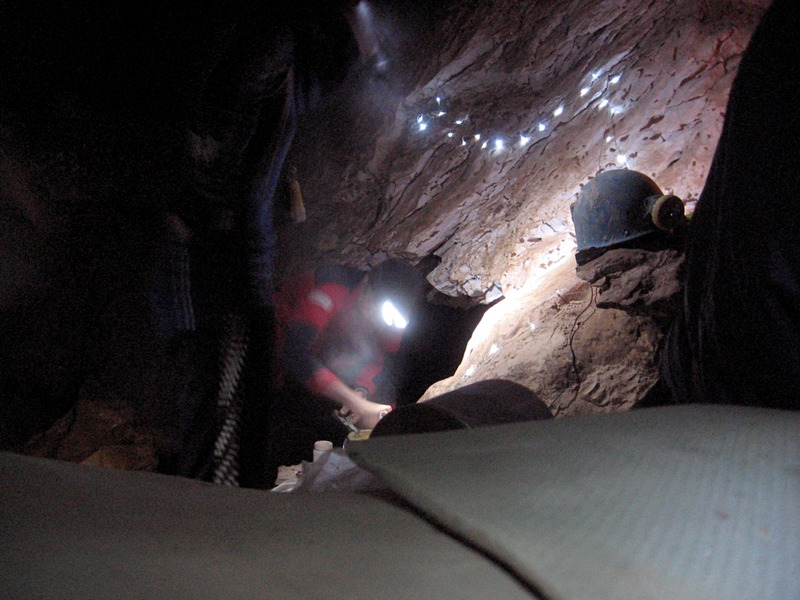
\includegraphics[width = \textwidth]{2011/ug_logbook/58.png}

{[}2011-07-31-01.11.35-Jarvist M Frost-CanonA520-IMG\_0167 - Jana and
Tetely Cooking Lond Exposure{]}

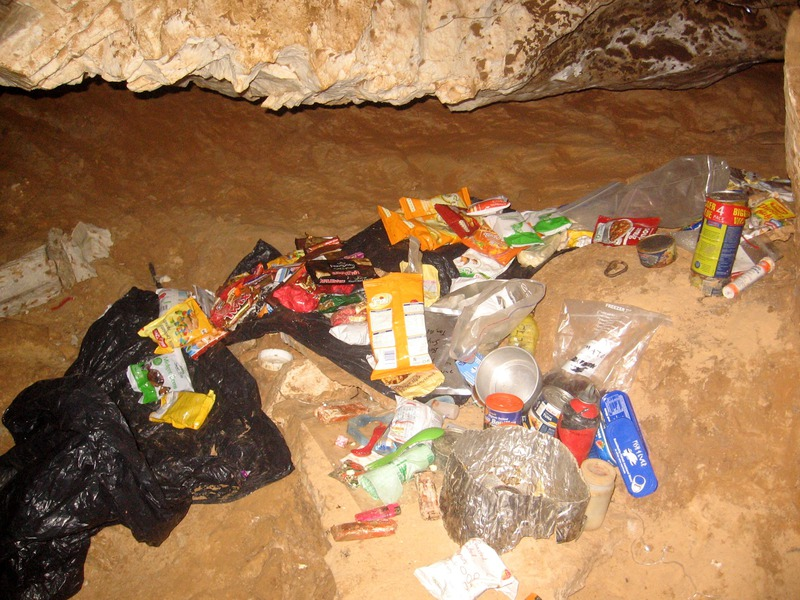
\includegraphics[width = \textwidth]{2011/ug_logbook/59.png}

{[}2011-08-01-13.24.46-Jarvist M Frost-CanonA520-IMG\_0175 - Food
Reserves and Stove at Camp \emph{X-Ray}{]}

{[}2011-08-01-13.24.09-Jarvist M Frost-CanonA520-IMG\_0173 - Dan
Drinking Tea in the Tent at Camp \emph{X-Ray}{]}

{[}2011-08-03-10.31.54-Grega-Panasonc DMC-FT2-105-camp \emph{X-Ray}{]}

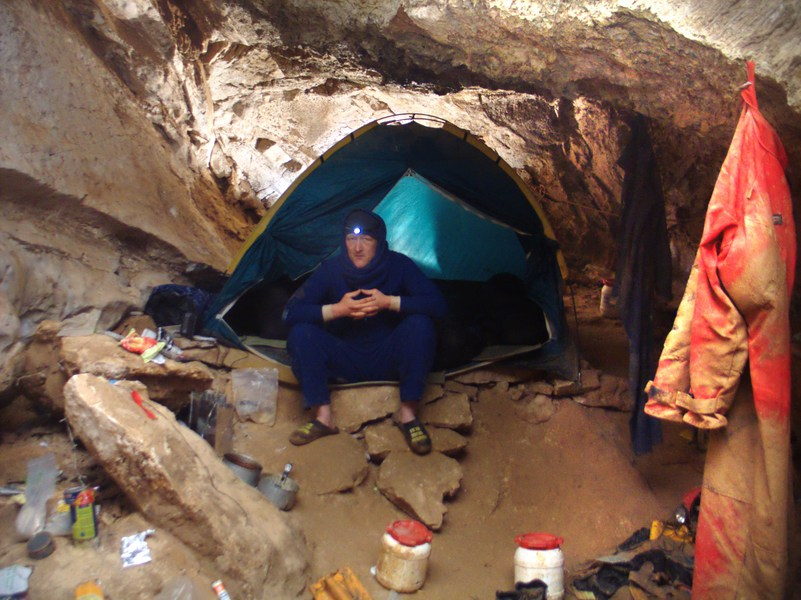
\includegraphics[width = \textwidth]{2011/ug_logbook/62.png}

{[}2011-08-07-12.10.52-Jarvist Frost-CanonG5-CRW\_0178 - jim at camp{]}

{[}Editor's note: Everything in square brackets has been added by
Tetley. I thought it was best to type up the writing; it took a lot
longer than I thought it would when I started but it's been good
reliving the memories! I've tried to keep original spelling etc., but a
few typos may have crept in -- sorry! Scan quality of drawings not the
greatest, again apologies. I added the photos to the document just for
the memories\ldots{}.May 2012{]}





2012 MOVED TO 2012-UGLOG.TEx - FIONA 28.10.23